\chapter{Proposed Architecture}\label{chap:propSol}

\section{Constituent Modules}

\subsection{Finite-precision representation system}
Before discussing any other details concerned with the actual hardware implementation, some of the design choices that were
made regarding how the numbers involved in the calculations are represented are laid out. For that purpose, Section~\ref{sec:precbit} discusses the fundamentals of fixed-point
representation systems, as well as the bitwidth and precision chosen for the number representation system of the network, and Section~\ref{sec:convrulesfp} states
how the conversion between real and fixed-point numbers is performed. Finally, Section~\ref{sec:arithrulesfp} explains the special rules that fixed-point arithmetic
imposes. The considerations made in this chapter can be found on~\cite{Yates13}, which is a good reference for fixed-point arithmetic theory.

\subsubsection{Precision bitwidth}\label{sec:precbit}
Since we are dealing with real numbers, and the plan is to make use of the DSP48 slices within the FPGA, an 18-bit signed fixed-point system was chosen, with the sign
information coded as 2's complement. Fixed-point systems are usually addressed in the $Qn.m$ form, where $n$ is the bitwidth of the of the integer part (excluding
the sign bit) and $m$ is the bitwidth of the fractional part, and so the total bitwidth is $N=m+n+1$ to account for the sign bit. In this way, the value of
the $i$-th position bit is $2^{i-m}$, and since this is a 2's complement system, the last bit is worth $-2^{n-1}$. In terms of range of representation, the maximum positive
number that can be represented corresponds to all bits set to one, except for the last ($2^{n+m+1}-1$), but shifted by $m$ bits to the right to yield the correct real
number (the decimal point is at the $m$-th bit), i.e.


\begin{equation}\label{eq:maxpos}
    \text{Max. Positive Number} = \frac{2^{N-1}-1}{2^m} = 2^{N-1-m} - \frac{1}{2^m}
\end{equation}
and the smallest negative number is simply the MSB set to one (and also shifted appropriately),

\begin{equation}\label{eq:minneg}
    \text{Small. Negative Number} = -\frac{2^{N-1}}{2^m} = -2^{N-1-m}.
\end{equation}

Assuming that the smallest perturbation used in the training system will be $2^{-9}$, according to the previous Python experiments, the fractional part precision should be,
at least, greater than this, so a sensible choice would be either $m=10$ or $m=11$. On the other hand, given that, in the Python experiments, it was attested that the
weight values generally do not (and should not) exceed values around the first power of ten, there is no need for large values of $n$ (although it is advisable to be large
enough to accommodate the intermediate calculations, avoiding overflow), and so we should choose to have as much precision as possible, so $m$ was set to 11. Since $18=n+m+1$, then
$n = 17 - m = 6$ and the representation system to be used is $Q6.11$. According to Equations~\ref{eq:maxpos} and~\ref{eq:minneg}, the real values $x$ than can be represented
with this choice of $n$ and $m$ are in the range

\begin{equation}\label{eq:rangeQ611}
    -64 \leq x \leq 63.99951172
\end{equation}
with a minimum resolution of $2^{-11} = 0.00048828125$.

\subsubsection{Conversion between real and fixed-point}\label{sec:convrulesfp}
In order to find the real number equivalent of a $Qn.m$ fixed-point system, and \textit{vice-versa}, we need to take into account that, according to
Section~\ref{sec:precbit}, the $i$-th position bit is worth $2^{i-m}$, and therefore the decimal point in this fixed-point system is at position $i=m$, since $2^{m-m} = 1$.
This way, the rules are as follows

\begin{itemize}
    \item \textbf{Positive Real to $Qn.m$} -- since the $1$ is at bit $m$, we simply multiply the real number by $2^m$, and discard the fractional part of the result
    \item \textbf{Negative Real to $Qn.m$} -- we disregard the sign in the real number, and perform the same operation as before, but we then convert the resulting binary number to two's complement, i.e. by performing bitwise negation, followed by summing 1.
    \item \textbf{Positive $Qn.m$ to real} -- multiply the fixed-point number by $2^{-m}$, to shift the decimal point back by $m$ positions.
    \item \textbf{Negative $Qn.m$ to real} -- convert from two's complement by performing bitwise logic negation, followed by summing one; then scale the decimal point back by $m$ positions by multiplying by $2^{-m}$.
\end{itemize}

\subsubsection{Fixed-point arithmetic rules}\label{sec:arithrulesfp}
The three main operations needed in my network design are \textbf{signed sums}, \textbf{signed multiplications} and \textbf{arithmetic shifts} (i.e. the ones that preserve the sign of the MSB)
to implement divisions/multiplications by powers of two. In terms of signed sums, the rule is simple: both numbers need to be scaled to the same base, with their $m$'s being same,
so that the decimal point is in the same place in both numbers ($n$, however, can be different, since that only means that one number is longer than the other, and the missing bits
in the smaller one are interpreted as zeros).

For signed multiplication, since both operands are in fixed-point $Qn.m$, and are thus scaled by $2^m$, we need to scale the result by multiplying it
by $2^{-m}$ (or perform an arithmetic right shift of $m$ bits). This is because, if $a$ and $b$ are the real numbers to be multiplied, and $c$ is the
result, we have that, in fixed-point arithmetic, the result is

\begin{equation}\label{eq:multfp}
    (a\cdot2^m) \cdot (b\cdot2^m) = c \cdot 2^{2m}.
\end{equation}
Since in $Qn.m$, all numbers are represented as $r 2^{m}$ with respect to their real counterpart $r$, we need to scale back the decimal point in the result of Equation~\ref{eq:multfp}. We can see
that it can be easily achieved by dividing by $2^m$, as stated in the previous paragraph.

\subsection{Activation Function Calculator}\label{sec:nonlincalc}
In order to evaluate the non-linear activation functions $\sigma(x)$ and $\tanh(x)$, since there is no algorithm that can directly compute them,
a suitable way to compute them accurately had to be found, using a finite number of elementary operations, multiplications and additions, that can be performed
efficiently by specially tailored blocks within the FPGA (DSP48 slices for multiplication, for instance). For that purpose, after using~\cite{Muller05} as a
reference on elementary function approximation algorithms, \textbf{Polynomial Approximations} were used, since evaluating a polynomial does not have high memory usage
needs (as opposed to Table Methods, for instance) and, if the polynomial degree is sufficiently low, the number of multiplications needed is low enough to not pose a restriction
both on resources (now DSP slices, and not memory) and in speed (number of number of clock cycles needed to output a result).

\subsubsection{Theoretical considerations on the approximation method}
The polynomial approximation methods aim to approximate some function $f(x)$ in an interval $\left[a, b\right]$ using a polynomial $p^*_n \in \mathcal{P}$ of
degree $n$, in order to meet the optimization criteria chosen \textit{a priori}. This optimization criteria can be either the
well-known \textbf{Least Squares Approximation} procedure, where we minimize the \emph{average quadratic error} $\left[f(x)-p^*(x)\right]^2$, or
the \textbf{Least Maximum Approximation}, where we \emph{minimize} the \emph{maximum possible error}, also commonly called a \textit{minimax} approximation.
Since we are operating in $Q6.11$ fixed-point arithmetic, we need to guarantee that the maximum approximation error is close to the precision limit of this
representation, $2^{-11}$, and so a \textit{minimax} approach is desirable, since it guarantees that a given maximum error is not exceeded. Weierstrass's
Theorem guarantees that there is always a polynomial that can approximate any continuous function f with error $\epsilon > 0$.
Chebyshev also proved~\cite{Muller05} that, in a \textit{minimax} polynomial approximation of degree $n$, the minimum approximation error $\epsilon$ is achieved in
at least $n+2$ points, and the sign of the approximation error alternates from one interval to the other, meaning that the error is not \emph{biased} and has zero average.
This leads to a linear system of $n+2$ equations, whose $i$-th line is given by

\begin{equation}\label{eq:remezline}
    p(x_i) - f(x_i) = (-1)^{n+1} \epsilon \Leftrightarrow p_0 + p_1 x_i + p_2 x_i^2 + \cdots + p_n x_i^n - f(x_i) = (-1)^{n+1} \epsilon
\end{equation}

The optimal coefficients of this \textit{minimax} polynomial are found using the \textit{Remez Algorithm}, which provides an iterative approach to solve the linear system given by Equation~\ref{eq:remezline} by finding, in each iteration, the $n+2$ set of points $x_i$ of Chebyshev's Theorem that minimize the error function to $\epsilon$. The algorithm operations are as follows

\begin{enumerate}
    \item Initializing the set $x_i$ of points to $x_i = \frac{a+b}{2} + \frac{(b-a)}{2}\cos\left(\frac{i\pi}{n+1}\right), \, 0 \leq i \leq n+1$
    \item Solve the system in~\ref{eq:remezline}
    \item Given the polynomial coefficients yielded by step 2, compute the $y_i$ points that minimize $p(x)-f(x)$, and replace the $x_i$s of the next iteration by these $y_i$s. Go to step 2 until $\epsilon$ does not decrease.
\end{enumerate}

On one hand, the system of~\ref{eq:remezline} of Step 2 can be written in matrix notation as

\begin{equation}
\begin{bmatrix} 1 & x_0 & x_0^2 & \cdots & x_0^n & - 1 \\ 1 & x_1 & x_1^2 & \cdots & x_1^n & + 1 \\  &  &  & \vdots & & \\ 1 & x_{n+1} & x_{n+1}^2 & \cdots & x_{n+1}^n & (-1)^{n+1} \end{bmatrix}
\begin{bmatrix} p_0 \\ p_1 \\ p_2 \\ \vdots \\ p_n \\ \epsilon \end{bmatrix} = \begin{bmatrix} f(x_0) \\ f(x_1) \\ \vdots \\ f(x_{n+1}) \end{bmatrix}
\end{equation}
and therefore the solution vector $p = \left[p_0 \; p_1 \; p_2 \; \cdots \; p_n \; \epsilon \right]$ for Step 2 of Remez's Algorithm is simply given by $p = A^{-1}b$, where $A$ is the matrix on the left-hand side of the equation and $b$ is the vector on the right-hand side. The Python implementation of this algorithm is presented in Listing~\ref{lst:remezpy} of Appendix~\ref{ap1:remez-pyth}.

Instead of using a \emph{single} polynomial of higher degree ($n \geq 3$) for the whole domain, the domain of the activation functions was partitioned
in \textbf{6 intervals}, and polynomials of degree $n=2$ were used to approximate the function in each of those intervals. This proved to yield a lower overall approximation error,
as expected (the interval on which to perform the approximation is smaller). Also, since both $\sigma(x)$ and $\tanh(x)$ have horizontal asymptotes
in $\{0,1\}$ and $\{-1,1\}$ respectively, the far-left and far-right intervals do not need a polynomial approximation, and can be assigned a constant value
equal to the corresponding asymptote. The resulting \textit{minimax} approximation polynomials yielded by running the code in Listing~\ref{lst:remezpy} are

\begin{equation}\label{eq:coefs_sigm}
\sigma(x) \approx \left\{
\begin{array}{lc}
0 & x  \leq -6 \\
0.20323428 + 0.0717631x + 0.00642858x^2 & -6 \leq x \leq -3 \\
0.50195831 + 0.27269294x + 0.04059181x^2 & -3 \leq  x \leq 0 \\
0.49805785 + 0.27266221x - 0.04058115x^2 &  0 \leq  x \leq 3 \\
0.7967568 + 0.07175359x - 0.00642671x^2 & 3 \leq  x \leq 6 \\
1 & x > 6
\end{array}
\right.
\end{equation}
for the sigmoid function and

\begin{equation}\label{eq:coefs_tanh}
\tanh(x) \approx \left\{
\begin{array}{lc}
-1 & x  \leq -3 \\
-0.39814608 + 0.46527859x + 0.09007576x^2 & -3 \leq x \leq -1 \\
0.0031444 + 1.08381219x + 0.31592922x^2 & -1 \leq  x \leq 0 \\
-0.00349517 + 1.08538355x -0.31676793x^2 &  0 \leq  x \leq 1 \\
0.39878032 + 0.46509003x - 0.09013554x^2 & 1 \leq  x \leq 3 \\
1 & x > 3
\end{array}
\right.
\end{equation}
for the hyperbolic tangent function. These constants were converted to $Qn.m$ using the rules in~\ref{sec:convrulesfp}, and embedded in the HDL model.

\subsubsection{Hardware Implementation}
The hardware module that implements these activation functions is, essentially, a 2nd degree polynomial calculator, where the coefficients of the polynomial are chosen accordingly with the value of the input $x$. This last functionality
is implemented using a simple multiplexer that loads the signals $p_0$, $p_1$ and $p_2$ with the coefficients of Equations~\ref{eq:coefs_sigm} and~\ref{eq:coefs_tanh} based on the value of the input operand $x$. As for the polynomial calculator is concerned, although we could use a full-pipelined evaluator, that would require two DSP slices -- to perform the two simultaneous multiplications -- but the DSP slices will be heavily used in the matrix-vector calculators, so it is advisable to save them for that purpose. A simpler approach is to note that, according to Horner's Rule, we get

\begin{equation}\label{eq:factorPol}
p(x) = p_0 + p_1x + p_2x^2 = p_0 + x(p_1 + xp_2)
\end{equation}
where we can note that this operation can be divided in a two-step procedure of a simultaneous multiplication of the operand by a constant,
and a subsequent addition of another constant: first, by multiplying the operand by $p_2$ and summing $p_1$, and then by multiplying the operand
by this last result and summing $p_0$. The block diagram of the hardware implementation of the non-linearity calculator is presented in Figure~\ref{fig:nonlin}.
Also, in Figure~\ref{fig:nonlin-out}, the output of the Verilog module that implements this design is compared with the actual output (Python3's Numpy was used as reference)
for both activation functions. The maximum error for the approximation of the $\sigma(x)$ was of 0.001408 and for the $\tanh(x)$ was 0.0121.

\begin{figure}
    \centering
    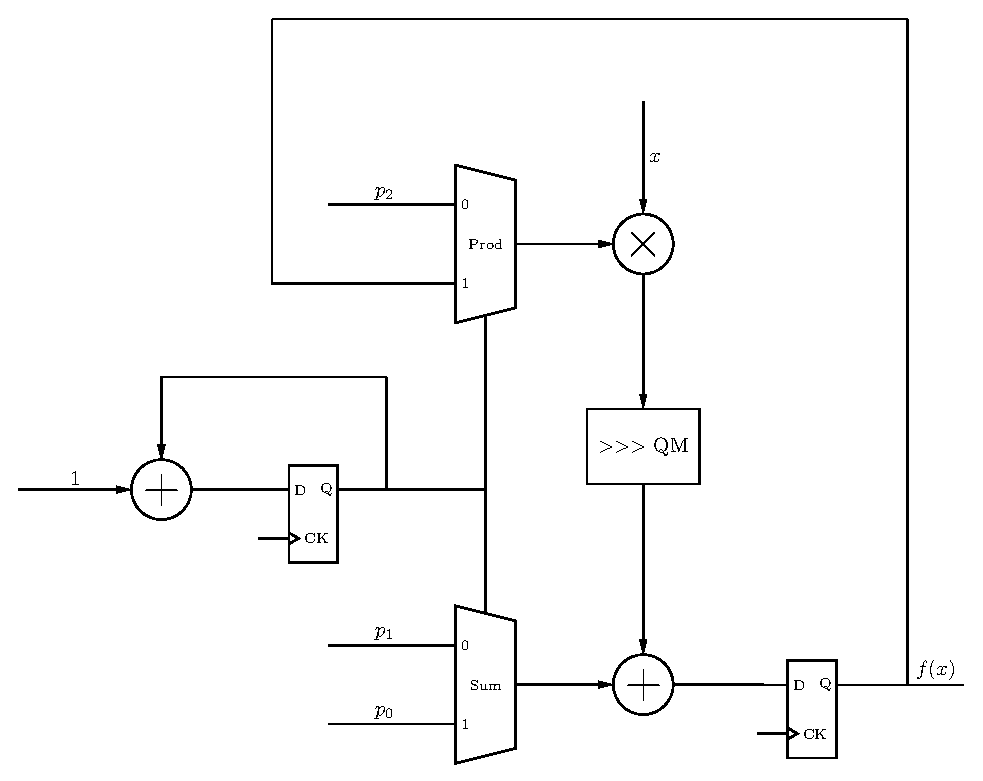
\includegraphics[width=0.9\linewidth]{figures/non-lin.eps}
    \caption[Block Diagram of the Activation Function Calculator]{Block Diagram of the Activation Function Calculator using a single multiplication. The multiplexer state is controlled by the flip-flip and sum block, that change state every clock cycle. When reset is applied, the selector is set to zero.}
    \label{fig:nonlin}
\end{figure}

\begin{figure}
    \centering
    \begin{subfigure}{0.85\linewidth}
        \centering
        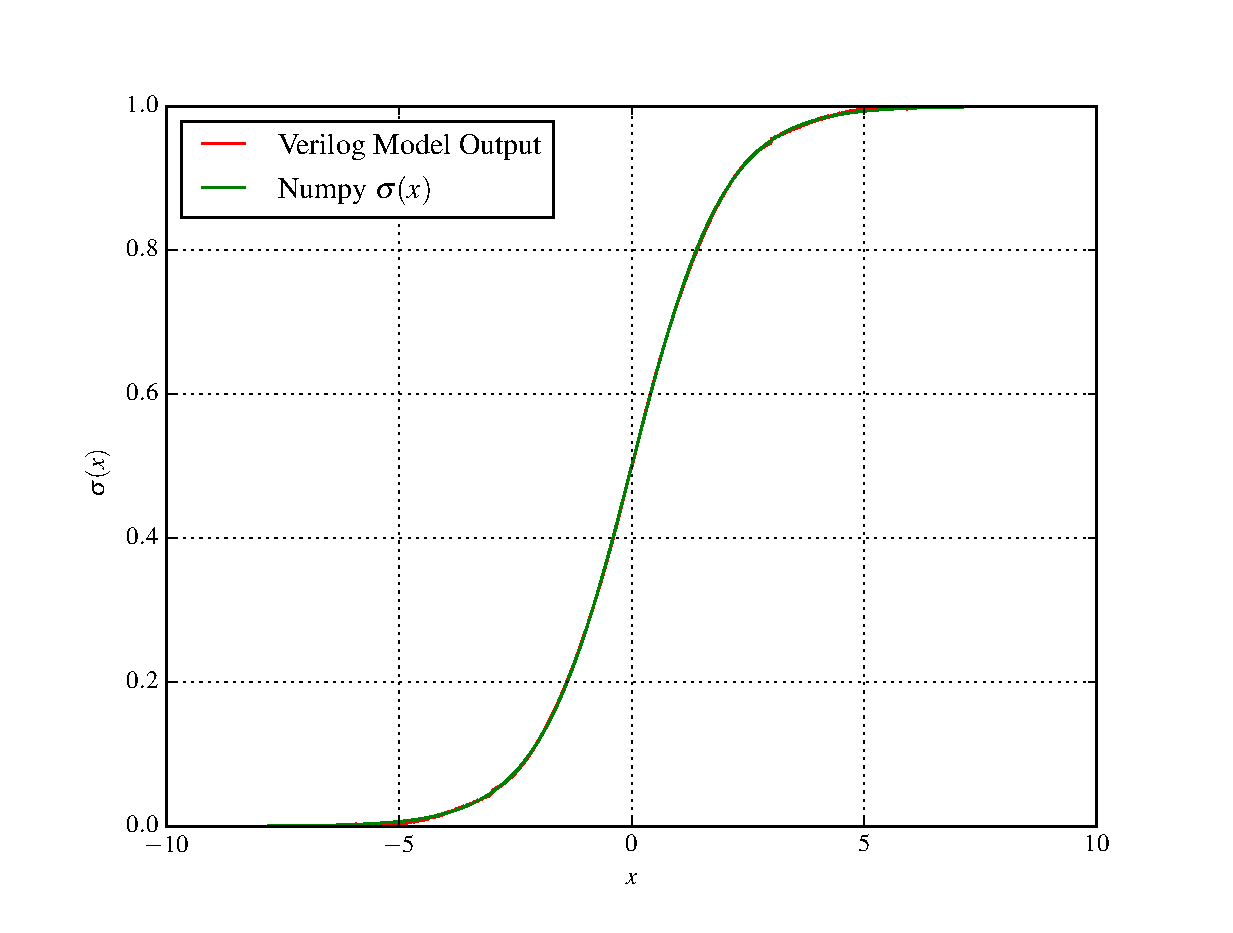
\includegraphics[width=\linewidth]{figures/nonlin-out.eps}
        \caption[Plot of the output of the Sigmoid Calculator HDL module]{Plot of the output of the Sigmoid Calculator HDL module}
        \label{fig:nonlin-out-sig}
    \end{subfigure}
    \begin{subfigure}{0.85\linewidth}
        \centering
        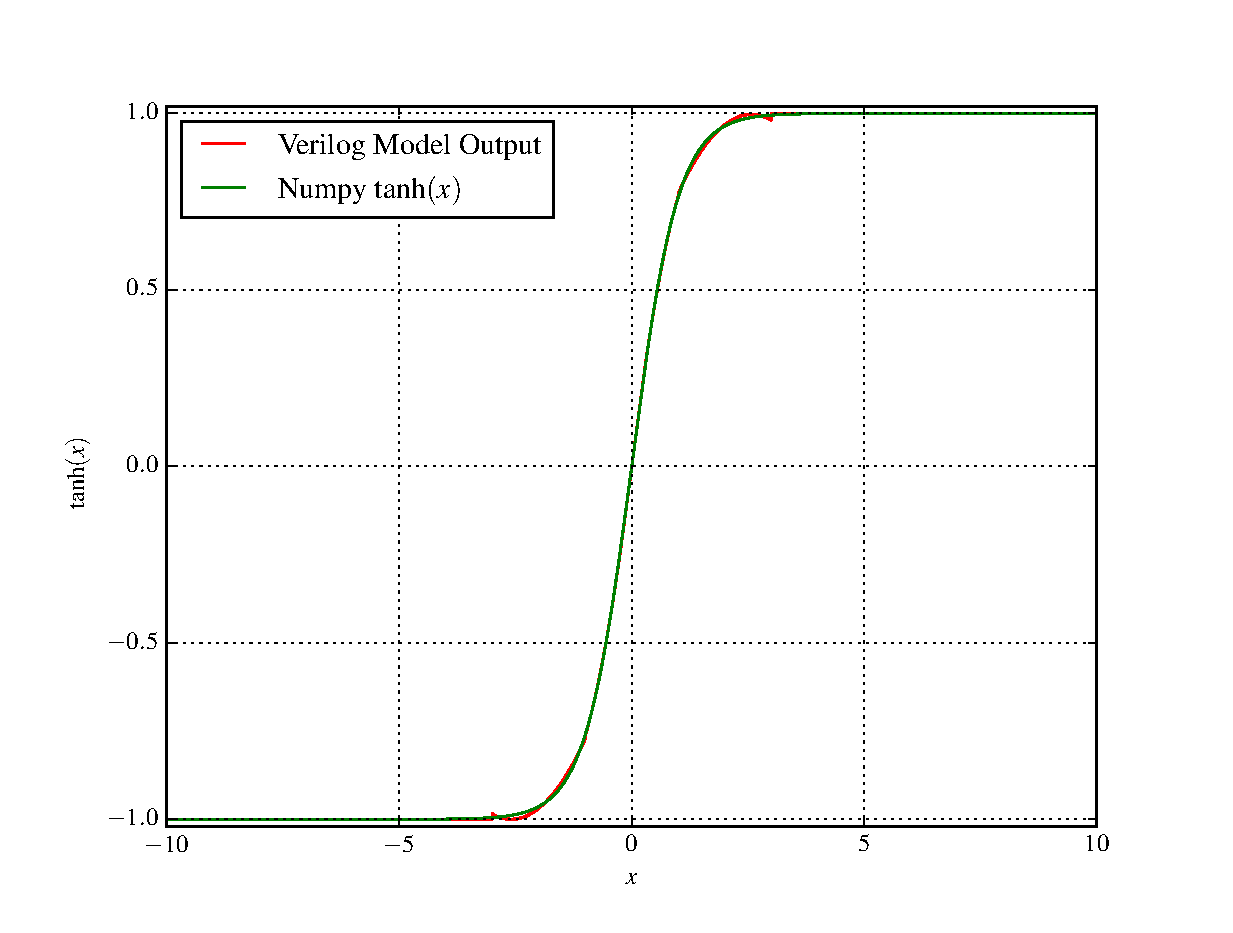
\includegraphics[width=\linewidth]{figures/nonlin-out-tanh.eps}
        \caption[Plot of the output of the Hyperbolic Tangent HDL module]{Plot of the output of the Hyperbolic Tangent HDL module}
        \label{fig:nonlin-out-tanh}
    \end{subfigure}
    \caption[The output of the HDL implementation of the activation functions]{The output of the HDL implementation of the activation functions}
    \label{fig:nonlin-out}
\end{figure}

\subsection{Matrix-vector Dot Product Unit}\label{sec:dotprod_sec}
From the set of Equations~\ref{eq:equationsLSTM}, we see that the weight matrices $\mb{W}_*$ and $\mb{R}_*$ are multiplied by the input
vector $\mb{x}$ and the layer output vector $\mb{y}$, respectively. This way, we need an HDL block that implements matrix-vector multiplication,
and the description of that block must be parameterized in order to accommodate different matrices/vectors of various sizes: note that $x$ has length $M$ (the number
of inputs to the layer), and so $\mb{W}_*$ has size $N\times M$, while $y$ has length $N$ (the number of neurons in the layer), and so $\mb{R}_*$
now has size $N\times N$. Plus, a layer with different parameters is needed, either in terms of number of inputs or number of neurons, it is advisable
to only change the respective parameter at the synthesis stage, instead of having to redesign the whole block for that particular size.

The matrix-vector dot product of a matrix $A$ of size $N \times M$ with a vector $\mb{x}$ of size $M$, if performed in a linear non-parallel way, can be described in terms of Algorithm~\ref{matvec-alg}

\begin{algorithm}
\begin{algorithmic}
\For {$i$ = $1:N$}
    \For {$j$ = $1:M$}
    \State $y_i := y_i + A_{ij} \cdot x_j$
    \EndFor
\EndFor
\end{algorithmic}
\caption{Matrix-vector multiplication of a matrix}
\label{matvec-alg}
\end{algorithm}
This operation has a computational complexity of $O(n^2)$. It can be seen that each of the $i$-th components of the output vector $\mb{y}$ can be calculated \textbf{in parallel},
each only requiring the corresponding $i$-th line from the matrix. Following this approach, matrix-vector multiplication can now be performed in \textbf{linear time}, which
is one of the great advantages of custom-tailored hardware solutions.

Although this solution only requires one multiplication per row of the input matrix (i.e. $N$ multiplications), if the row size is large, we may quickly run out of resources in the FPGA
as $N$ increases; therefore, some sort of \textit{resource multiplexing} strategy must be used to ensure the flexibility of the solution to accommodate networks of larger dimensions.
The solution found for this issue was to \emph{share} the multiplication slice between rows of the matrix: in a direct implementation of Algorithm~\ref{matvec-alg}, each
multiplication slice was responsible for producing the $i$-th element of the output vector $\mb{y}$ (of size $N$), therefore the final result for the vector would be ready in $M$
clock cycles (i.e. the number of columns); now, if defining a parameter $K_G = \frac{\text{Number of rows}}{\text{Number of multipliers}}$, the number of rows that share the
same multiplier, each multiplier is responsible for producing several $i$-th elements of the output vector, in consecutive time slots of $M$ clock cycles. Suppose that we
have a $8\times2$ matrix, and that $K_G = 2$; in this way, we would have 4 multipliers, and the output vector elements $y_0$, $y_2$, $y_4$ and $y_6$ would be ready after $M=2$
clock cycles, and the remaining -- $y_1$, $y_3$, $y_5$ and $y_7$ --  are ready after another two clock cycles, that is $2M = 4$ clock cycles after the calculations began.

Figures-\ref{fig:mem-arrayprod} and~\ref{fig:array-prod} depict a diagram of the memory access for the Matrix, and the row multiplication units within the module, respectively,
where $K_G = 4$ was set, for the same matrix and vector sizes as before. Note that in this situation there would be only 2 multipliers, and therefore the module would be composed of two
multiplication units, such as those in Figure~\ref{fig:array-prod}, that work in parallel: they address a particular column using the signal \verb+colSel+, which is used by the RAM
module to output the corresponding column of the matrix (in regard to the input vector, obviously this signal selects only a single position), depicted in Figure~\ref{fig:mem-arrayprod}.
The dark shaded part of the memory is used by the first multiplier, and the light shaded is used by the other, in parallel for a fixed \verb+rowMux+ -- this signal is produced by the
control unit of the module, and essentially operates the left Mux and right Demux of Figure~\ref{fig:array-prod} that allows to choose the proper position of the weight column and to
write to the correct output register, respectively. In this example, for \verb+rowMux+=0, the control unit increments \verb+colSel+ from 0 to $M$, and thus evaluating $y_0$ and $y_4$.
After this, \verb+rowMux+ is incremented to 1, and the process repeats until \verb+rowMux+ reaches $K_G-1$. Therefore, we have the correct result vector in a time proportional to $K_G \cdot M$:
since the memory only outputs the appropriate column in the \emph{next clock cycle}, and that this module is pipelined both at the input and at the output in order to increase the maximum clock
frequency, we should add a 3 clock cycle overhead to the previous estimate.

\begin{figure}
    \centering
    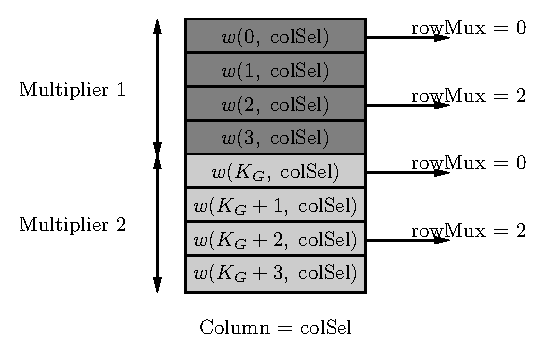
\includegraphics[width=0.9\linewidth]{figures/mem-array-prod.eps}
    \caption[A column of the matrix that serves as input to the module]{A column of the matrix that serves as input to the module. The dark shaded part is for the first multiplier, and the light shaded is for the other, in parallel. The rowMux signal addresses the position within each shaded area}.
    \label{fig:mem-arrayprod}
\end{figure}

\begin{figure}
    \centering
    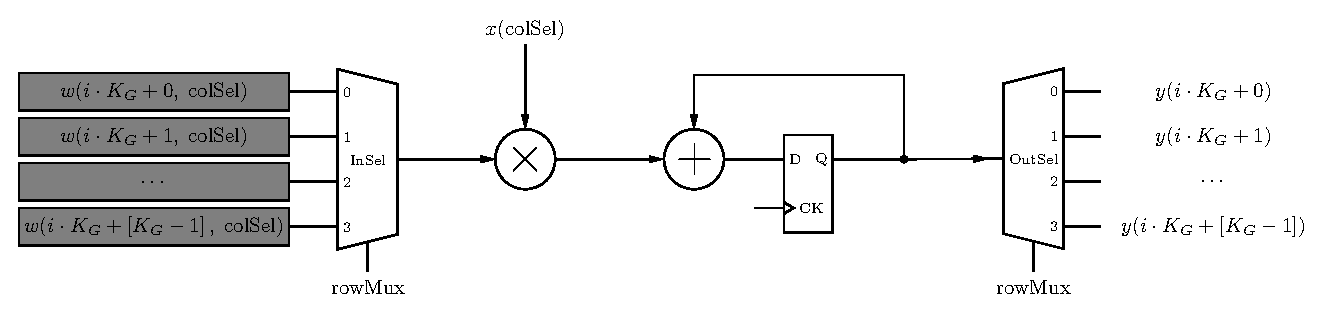
\includegraphics[width=\linewidth]{figures/array-prod.eps}
    \caption[The $i$-th row multiplication unit of the Module]{The $i$-th row multiplication unit of the Module, where rowMux and colSel are internal signals produced by the control unit of the module. The flip-flop accumulates the sum, and the output Demux selects the appropriate memory position on where to store this value, within the slot attributed to this multiplication, from $i\cdot K_G$ to $i\cdot K_G + \left[K_G-1\right]$}
    \label{fig:array-prod}
\end{figure}


\subsection{Dual-port weight RAM}
Even though bias weight vectors, with size $N\times 1$, were kept as normal registers and the synthesis tool was left to decide how to place them in the FPGA,
for the weight matrices the case is different. Since the network size can be large, it is good to make sure that they are placed in the RAMs available
in the FPGA. In Section~\ref{sec:dotprod_sec} we see that, because of the architecture of the matrix-vector multiplier, it is convenient to have a column
by column access to the weight matrix, and therefore this block was designed to output a given column in the \verb+rowOut+ output port terminal, at the \emph{positive edge} of
the clock, selected by the value present in the input \verb+addressOut+ at the immediately previous \emph{positive edge} of the clock. As far as \textbf{writing} to
the memory is concerned, the process is identical but now the column of weights at the input \verb+rowIn+ is sampled at \emph{positive edge} of the clock, and is placed
at the column specified by the input \verb+addressIn+ at the previous \emph{positive edge} of the clock.

Note that, for an $N \times M$ matrix, since the memory outputs and writes one column at a time, both the input and output port terminals will carry $N$ weights,
and a total bitwidth of $\verb+BITWIDTH+ \cdot N$.

The Verilog coding followed the Verilog Coding Guidelines in Xilinx's \href{http://www.xilinx.com/support/documentation/sw_manuals/xilinx2015_2/ug901-vivado-synthesis.pdf}{UG901 Document} that,
in page 50, recommends that the \verb+RAM_STYLE+ parameter be set to \verb+block+. This can be done by adding the following compiler directive before the register definition, as follows

\begin{verbatim}
(* ram_style = "block" *) reg [PORT_BITWIDTH-1:0] RAM_matrix [NCOL-1:0];
\end{verbatim}
where we can see that each register contains the respective column of the matrix, with $\verb+PORT_BITWIDTH+ = \verb+BITWDITH+ \cdot M$ and $\verb+NCOL+ = M$.

After performing synthesis, it was noticed that using block RAM led to a slightly poorer speed performance, so I have settled with the use of \emph{Distributed RAM}, storing the weight matrices in LUTRAM.


\subsection{Gate Module}\label{sec:gatemod}
The Gate modules are responsible for producing the internal signal vectors for $\mb{z}^{(t)}$, $\mb{i}^{(t)}$, $\mb{f}^{(t)}$ and $\mb{o}^{(t)}$. If we note that, according
to~\cite{Greff15}, the removal of peepholes (the signals $\mb{p}_*$) does not compromise significantly the performance of the network~\ref{sec:struct_lstm}, they were omitted
in order to simplify the Gate Module and reduce the usage of DSP slices. This way, a Gate module needs to perform three tasks

\begin{enumerate}
    \item Multiply matrix $\mb{W}_*$ by the input vector $\mb{x}^{(t)}$
    \item Multiply matrix $\mb{R}_*$ by the previous layer output vector $\mb{y}^{(t-1)}$
    \item Sum the bias vector $\mb{b}_*$ to the remaining matrix-vector dot product results.
\end{enumerate}
Assuming that the network size $N$ is always larger than the input size $M$, if we use the matrix-vector dot product units of Section~\ref{sec:dotprod_sec}, the multiplication in task 1 takes approximately $K_G\cdot M$ cycles and the one in task 2 takes $K_G\cdot N$ cycles. This way, task 2 and task 1 can be performed in parallel, and we can use the extra time that task 2 takes, relative to task 1,  to perform task 3, and sum the bias vector to the output of task 1, whose result is ready by that time. The module is triggered by a \verb+beginCalc+ input signal that activates the internal state machine, and outputs a \verb+dataReady+ signal that informs the network that the calculations have been concluded, and the value at the output is the actual final result.
After validating and simulating this block, and taking into account the internal state-machine and that the internal datapath is pipelined, the exact number of clock cycles this
module takes to output a result is $6+K_G\cdot N$.

\begin{figure}
    \centering
    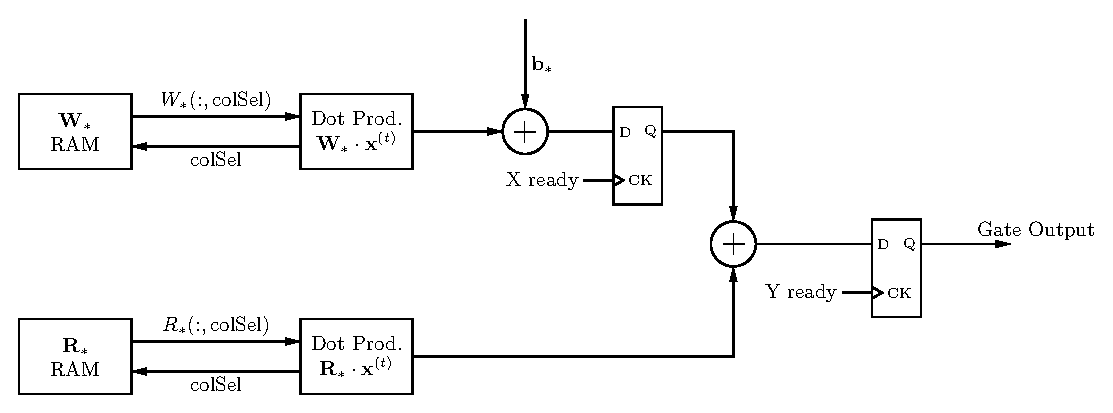
\includegraphics[width=\linewidth]{figures/gate.eps}
    \caption[Diagram of the hardware block that implements the Gate]{Diagram of the hardware block that implements the Gate}
    \label{fig:gate}
\end{figure}

\section{Hardware LSTM Network -- Forward Propagation}\label{sec:hLSTM-fp}
After detailing the design of each of the constituent modules of the LSTM Network, it will now be shown how they are interconnected
to implement a hardware version of Equations~\ref{eq:equationsLSTM}. This is performed in Section~\ref{sec:hLSTM-struct}, where the design decisions
and compromises that were taken are detailed, along with some estimates on the resource usage and calculation time for each of the design iteration versions, namely
the \textit{naïve solution} (~\ref{sec:struct-fullpar}) and an \textit{optimized version} of the former (~\ref{sec:struct-shared}) that exploits some
of the hardware redundancies by multiplexing in time the usage of those redundant structures.

\subsection{Network Structure}\label{sec:hLSTM-struct}
Looking at Equations~\ref{eq:equationsLSTM}, we note that the signals $\mb{z}^{(t)}$, $\mb{i}^{(t)}$, $\mb{f}^{(t)}$ and $\mb{o}^{(t)}$ do not depend on each other, because
they operate only on the current input vector $\mb{x}^{(t)}$ and the previous layer output $\mb{y}^{(t-1)}$. This way, they can be calculated in parallel, meaning that we need
four Gate Modules (see Section~\ref{sec:gatemod} working in parallel, each one with its respective two RAMs for $\mb{W}_*$ and $\mb{R}_*$, and followed by the respective activation
function calculator (detailed in Section~\ref{sec:nonlincalc}), \textbf{one for each} of the $N$ vector elements. There are three elementwise multiplications, two for producing
signal $\mb{c}^{(t)}$ (which can be done in parallel and then summed elementwise) and one for $\mb{y}^{(t)}$ (which can be done only after applying the activation function $\mb{c}^{(t)}$).

\subsubsection{Fully Parallel}\label{sec:struct-fullpar}
By implementing directly the ideas outlined previously, we get the network of Figure~\ref{fig:network}. The memory element of the network is the array of flip-flops that
keep the value of the vector $\mb{c}^{(t)}$, which is activated every time we have a new incoming signal in order to store the last value, which is now $\mb{c}^{(t)}$

In terms of DSP slice usage, this proposed design comprises 3 elementwise multiplications and 5 activation function Modules. Since the number of elementwise multiplications is
equal to the network size $N$, we need $3N$ DSP slices for each elementwise block. As far as the activation function module is concerned, since we need to apply it to each one
of the $N$ elements of the Gate's output vectors, and each module uses one multiplication, the ensemble of all 5 modules needs $5N$ DSP slices. Therefore, and noting that each
Gate has $\frac{2N}{K_G}$ DSP slices, the total number of DSP slices used is

\begin{equation}\label{eq:numdsp_network}
    4\frac{2N}{K_G} + 5N + 3N = N \left( \frac{8}{K_G} + 8 \right).
\end{equation}
In terms of time performance, we can measure it by estimating the number of clock cycles needed to perform a complete forward propagation. Since the gate module
outputs a result in $K_G \cdot N + 7$ cycles, the activation function evaluators need always 5, and the elementwise multipliers need only 2 cycles (one cycle
for the pipeline, and another for the actual calculation), and noting that the two elementwise multipliers that sum to produce $\mb{c}^{(t)}$ can work in parallel,
the estimated number of clock cycles needed would be proportional to

\begin{equation}\label{eq:numcc_network}
    (N \cdot K_G + 6) + (5 + 2) + (5 + 2) = 20 + N\cdot K_G
\end{equation}

\begin{figure}
    \centering
    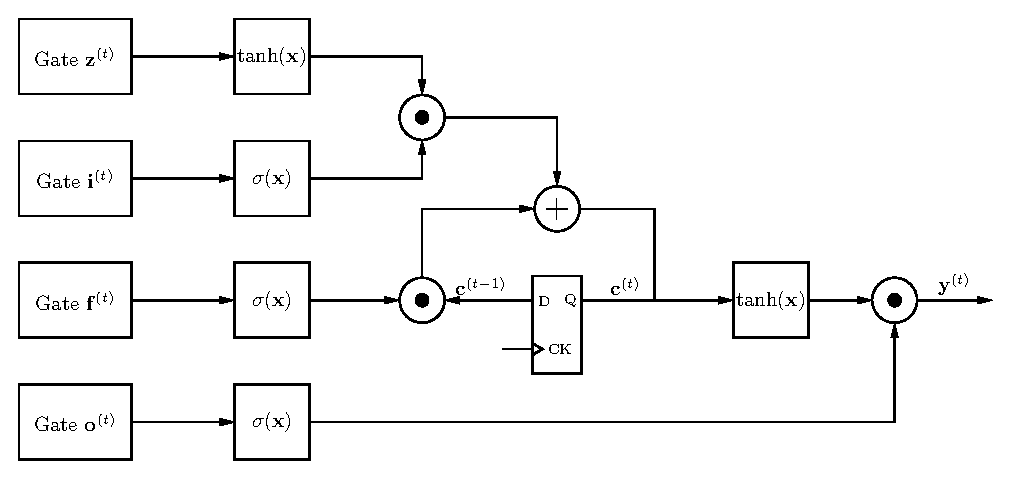
\includegraphics[width=0.9\linewidth]{figures/network.eps}
    \caption[Hardware LSTM Network with full level of parallelism]{Hardware LSTM Network with full level of parallelism}
    \label{fig:network}
\end{figure}

\subsubsection{Shared Elementwise Multiplication Block}\label{sec:struct-shared}
In Figure~\ref{fig:network}, we see that, apart from the elementwise multiplier preceding the register, all of them follow a similar structure: one of the
operands is the output of a $\tanh(\mb{x})$ block and the other from a $\sigma(\mb{x})$. An improvement over the last network architecture is to, instead of
replicating these `$\tanh$-$\sigma$-$(\cdot)$wise' structures, use a \emph{single one} and choose the input operands accordingly to the state that the network is
currently in. Besides, the right elementwise multiplier of Figure~\ref{fig:network} is not used as the same time as any other, so it is a waste of resources.
The issue about the elementwise multiplier that precedes the register can be solved by adding another multiplexer that chooses between the output of the $\tanh(\mb{x})$
module or the signal $\mb{c}^{(t-1)}$. These ideas resulted in the improved network design of Figure~\ref{fig:network-opt}.

\begin{figure}
    \centering
    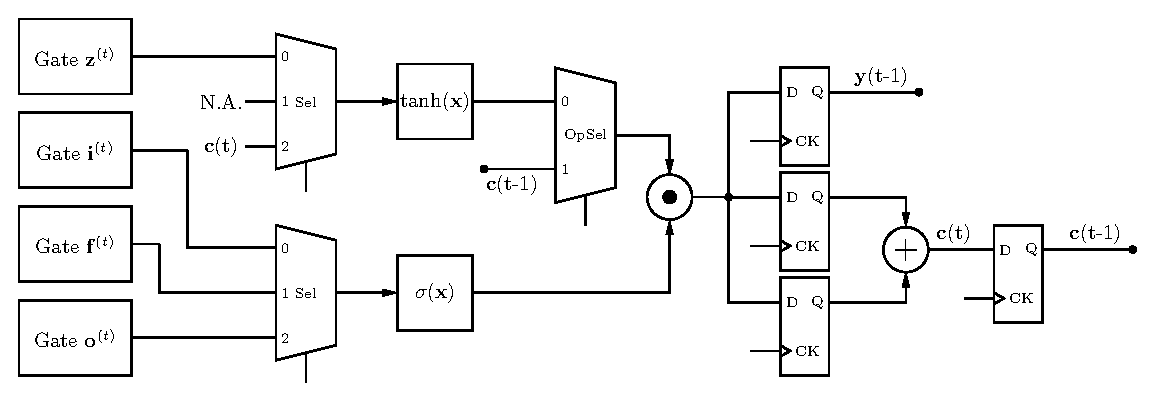
\includegraphics[width=0.9\linewidth]{figures/network-opt.eps}
    \caption[Optimised version of~\ref{fig:network} that shares the elementwise multiplication and the activation function blocks]{Optimised version of~\ref{fig:network} that shares the elementwise multiplication and the activation function blocks}
    \label{fig:network-opt}
\end{figure}
The two left multiplexers control the operands that are fed to the activation function modules, and the selecting signal is generated by the network's state machine and its value
is incremented after each complete usage of the `$\tanh$-$\sigma$-$(\cdot)$wise' structure: this is where the time multiplexing of the structure takes place.
Since in state $\verb+Sel+=1$ the left operand of the elementwise multiplier (the one that preceded the register in the previous design) is the signal $\mb{c}^{(t-1)}$,
another multiplexer was added before the elementwise multiplication, that selects that signal in that particular case, and the output from the $\tanh(\mb{x})$ block otherwise.

The registers on the right hand side of Figure~\ref{fig:network-opt} are activated by signals generated within the network state machine that enable the appropriate
register, placing the output from the elementwise multiplicator in the correct place. The first activated register is the middle one, which keeps the result from the
operation of the $\mb{z}^{(t)}$ and $\mb{i}^{(t)}$ vectors, then, after a full operation of the elementwise multiplier, the bottom register is enabled to save the other portion of
the sum that evaluates to the $\mb{c}^{(t)}$ signal. Lastly, the top register saves the network output $\mb{y}^{(t)}$, which in the next incoming sample becomes $\mb{y}^{(t-1)}$
and is used by the Gate modules in this next batch of calculations.

Now, since there is only a single elementwise multiplier and only two activation function calculators, the total requirement for DSP slices is simply
\begin{equation}\label{eq:numdsp_network-opt}
    4\frac{2N}{K_G} + 2N + N = N \left( \frac{8}{K_G} + 3 \right).
\end{equation}
where we see that we saved $5N$ multipliers when comparing to the previous design, which for a large value of $N$ can have a decisive impact.
In terms of speed performance, although the Gate calculation time remains the same, now the `$\tanh$-$\sigma$-$(\cdot)$wise' structure runs
for 3 consecutive times, in a non parallel fashion. After adjustments to the state machine, and accounting for pipelining and synchronization
within the datapath, the clock cycles needed after the gate calculations are 27, so the total clock cycles needed are

\begin{equation}\label{eq:numcc_network-opt}
    (N \cdot K_G + 6) + 27  = 33 + N\cdot K_G
\end{equation}
which is only 13 clock cycles more than the fully-parallel architecture. For instance, an $N=32$ neuron network using the fully-parallel design would require 320 DSP slices,
while this new architecture would only require 160. Only at the expense of 13 clock cycle overhead.

\section{Hardware LSTM Network -- SPSA Training}
In this section, a digital circuit is proposed that aims to train the Network whose details were explained in the previous Section by implementing the training
algorithm of Section~\ref{sec:training_lstm}. The training consists in changing the weight values in the RAMs accordingly with the error of the current prediction
against the correct outcome. This involves \textbf{two} forward propagations: one, where we run the network with the weights unchanged, and another where we \emph{perturbate}
the weights by a parameter $\pm \beta$ (the actual sign for each weight is generated at the beginning of the first forward propagation). After these two forward propagations,
there is a small time frame where the weights are updated, row by row, before the next incoming sample. This is explained in Section~\ref{sec:train-circ}. The way how the numbers
are randomly generated in hardware is presented in Section~\ref{sec:randnum-circ}.

\subsection{Pseudo-random Number Generator}\label{sec:randnum-circ}
While a True Random Number Generator (TRNG) generates data from a physical entropy source, a Pseudo-random Number Generator (PRNG) generates a sequence of numbers by applying a given
function, consecutively, to an initial seed. This means that, if one knows that initial seed and the function that generates the sequence, one can predict the previous and
future numbers given the current state. While this is not acceptable for high security cryptographic systems, it serves the purpose of providing a sequence of random sign
vectors (from whom both the signal of the perturbation and the update will be chosen from). The remaining issue is to find a PRNG with good statistical qualities, so instead
of implementing a simple linear-feedback shift register (LFSR), I did some research on the topic, and eventually chose the solution of~\cite{Tkacik2003}, based on a 43-bit LFSR
and a 37-bit Cellular Automata, by selecting 32 bits from each, permuting the bits and performing a bitwise XOR -- the output has, also, 32 bits. The quality of the
statistical properties are guaranteed, since it passed the DIEHARD test battery, as well as others, according to~\cite{Tkacik2003}.

\begin{figure}
    \centering
    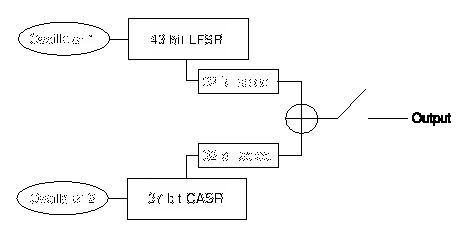
\includegraphics[width=\linewidth]{figures/prng.eps}
    \caption[The 32 bit Pseudo-random Number Generator. Source~\cite{Tkacik2003}]{The 32 bit Pseudo-random Number Generator. Source~\cite{Tkacik2003}}
    \label{fig:prng}
\end{figure}
The generator polynomial of the LFSR is a maximal length polynomial, $x^{43}+x^{41}+x^{20}+x+1$, and thus has a period equal to $2^{43}-1$. The CA is also a register, but each bit is updated
according to a given \textbf{rule} based on the values of the neighboring bits. This particular CA follows Rule 150 for the bit in position $i=27$, given by $c_{t+1}(i) = c_{t}(i-1) + c_{t}(i) + c_{t}(i+1)$, and
the remaining bits are updated by Rule 90, given by $c_{t+1}(i) = c_{t}(i-1) + c_{t}(i+1)$. The bits positioned at the borders also follow rule 90, but treat as zeros the non-existing $i$ positions.

The output of the hardware implementation of this PRNG is presented in Figure~\ref{fig:prng_out}. It is a state-time diagram, where the contents of the
registers at each time are represented by black (ones) and white (zeros). Tthe left column represents the output of the LFSR, the center column is the
output of the Cellular Automata and the right column is their combined output. As one can see, the time dependence of the LFSR is very high, which is not desirable.
The Cellular Automata, although uncorrelated, still retains some of the patterns that emerge from CAs. On the other hand, the combined output is the one that most resembles
white noise, which is a desirable characteristic.

\begin{figure}
    \centering
    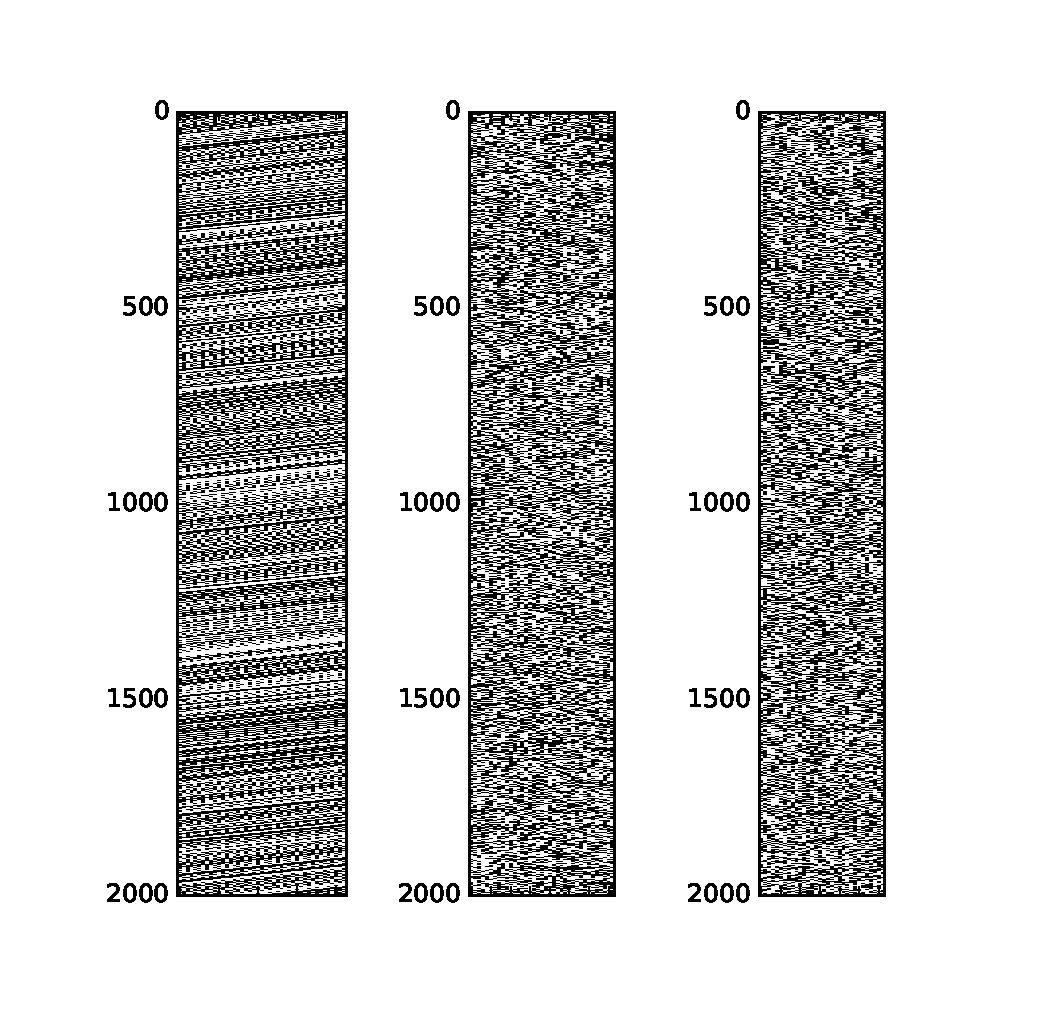
\includegraphics[width=\linewidth]{figures/prng_out.eps}
    \caption[The output of the implementation of the presented PRNG (right). The LFSR is the left column, and the CA is at the center]{The output of the implementation of the presented PRNG (right). The LFSR is the left column, and the CA is at the center. The zeros are represented by white, and the ones by black}
    \label{fig:prng_out}
\end{figure}



\subsection{Training Algorithm Circuit}\label{sec:train-circ}
Here is presented the proposed digital circuit of the SPSA training for the network. The circuit of Figure~\ref{fig:train} is replicated for each of the
eight weight RAMs, and the Sign RAM holds a single bit for each of the weight positions of the weight RAMs. This bit keeps the sign of the perturbation
to be applied to that particular weight, both on the second forward propagation and on the training stage. During the first forward propagation, and since
the weights are not perturbed in this run, we can use this time to populate the sign RAMs with new values for the next training stage, coming from the
PRNG of Section~\ref{sec:randnum-circ}. For this purpose, the PRNG is activated by the signal \verb+genRandNum+, generated by the state machine, and we
write columns of bits to the sign RAM, re-using the addressing signal produced by the Gate, namely \verb+colAddressRead+ (\verb+weightUpdate+ is set to
zero at this stage). At the second forward propagation, \verb+pertWeights+ is set to one, and the Perturbation Mux selects the input where the weights
are summed with the perturbation $\beta$, whose sign is selected by the sign RAM.

After this stage is completed, and before the network starts a new training cycle for the new incoming sample, we perform the actual training. For that purpose,
\verb+weightUpdate+ is set to one, and we enable writing to the Weight RAM. Also, the machine state is now responsible for addressing both RAMs, and we
begin a simultaneous \emph{pipelined} write to the Weight RAM: this is done by delaying the Write address in respect to the Read address by one clock cycle. This way, at
the first clock cycle, while we read Column 0, the next clock cycle will read Column 1 \emph{and} write the sign-changed column 0 plus the update coming
from the difference between the outputs in the two forward propagations. In order to simplify the update rule of Equation~\ref{eq:spsa_updateRule},
$\alpha$ and $\beta$ were fixed to negative powers of two, and this replaces the multiplication and division by a simple arithmetic right shift -- this idea
is also proposed by~\cite{Maeda05} -- considerably simplifying the design.

\begin{figure}
    \centering
    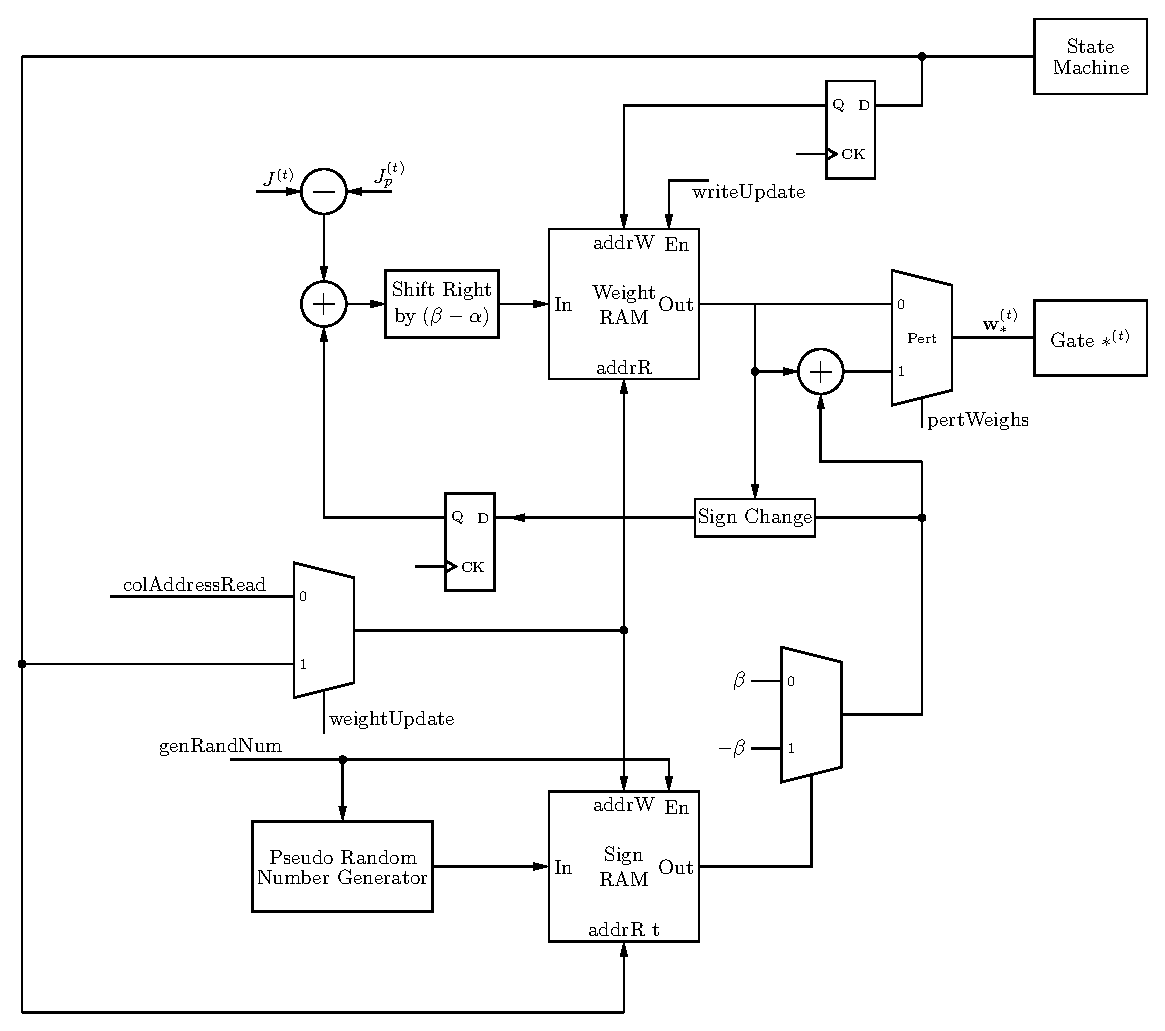
\includegraphics[width=\linewidth]{figures/train.eps}
    \caption[Proposed Hardware Implementation of SPSA Training]{Proposed Hardware Implementation of SPSA Training}
    \label{fig:train}
\end{figure}
